
\documentclass[a4paper, 12pt, notitlepage]{report}

\usepackage{amsmath, amssymb, amsfonts, amsthm}
\usepackage{cite}
\usepackage{graphicx}
%\graphicspath{ {/images} }

\title{Binary Segmentation}
\author{Louis Forbes Wright}
\date{\today}

\newtheorem{theorem}{Theorem}[chapter]
\newtheorem{lemma}[theorem]{Lemma}
\newtheorem{corollary}{Corollary}[theorem]

\begin{document}
\maketitle

%citation example. \cite{Venk}


%We are interested in the problem of seperating the signal from noise in a given dataset. How do we do this?

%Section 1 is an introduction the problem 
%Section 2 defines and expands some useful definitions we will be using
%Section 3 focuses on the theorem of Binary Segmentation and its associated lemmas
%Section 4  looks at an algorithm based on the theorem and from monte carlo simulations how consistent it is 
%Section 5 applies the theorem to some actual data collected from ...

%\bibliography{mybib} { }
%\bibliographystyle{plain}


%%%%%%%%%% PRELIMINARY MATERIAL %%%%%%%%%%
%\maketitle
\begin{center}
A project of 20 credit points at level 4. % change this
\\[12pt]
Supervised by Dr.\ Haeran Cho. 
\end{center}
\thispagestyle{empty}
\newpage
\section*{Acknowledgement of Sources} % this must be included in undergradate projects
For all ideas taken from other sources (books, articles, internet), the source of the ideas is mentioned in the main text and fully referenced at the end of the report.

All material which is quoted essentially word-for-word from other sources is given in quotation marks and referenced.

Pictures and diagrams copied from the internet or other sources are labelled with a reference to the web page or book, article etc.
\\[12pt]
Signed \dotfill Date \dotfill

\newpage
\section*{Abstract}
We are interested in the problem of seperating the signal from noise in a given dataset. How do we do this?
we are interested in the consistent estimation of the number and location of change-points and means in the a fixed sample.
\begin{itemize}
\item[] Section 1 is an introduction the problem
\item[] Section 2 defines and expands some useful definitions we will be using 
\item[] Section 3 focuses on the reinterpreting the theorem of Binary Segmentation and its associated lemmas 
\item[] Section 4  looks at an algorithm based on the theorem and from monte carlo simulations how consistent it is \cite{Venk}
\item[] Section 5 applies the theorem to some actual data collected from ... \cite{fryzlewicz2018}
\end{itemize}
Many thanks to ... who is the inspiration and source of many of the results within this work \cite{fryzlewicz2014}.


\tableofcontents 

%%%%%%%%%% MAIN TEXT STARTS HERE %%%%%%%%%%

%%%%%%%%%% SAMPLE CHAPTER %%%%%%%%%%
\chapter{Introduction}
%
"A change-point is a point after which the stochastic behaviour of a process changes" 
 Let.

\chapter{Definitions}
%

\section{Formalisation of the problem }

More formally "A multiple change-point problem deals with processes having more than one change-point. Our problem of interest is the consistent estimation of the number and the locations of the change-points. The problem is described more precisely below. 

Let \( {X_i ^{(n)} ;1 \leq i \leq n < \infty} \) be an array of random variables (vectors) and let $F^{(n)}_i$ be the distribution function of the random variable (vector) $X^{(n)}_i$. Let the $n^{th}$ of the array have $m_n$ change-points, that is, there exist \( \nu^{(n)}_1, \cdots, \nu^{(n)}_{m_n} \), where  \(0 =  \nu^{(n)}_0 <  \nu^{(n)}_1 < \cdots < \nu^{(n)}_{m_n} < \nu^{(n)}_{m_{n+1}} = n\), and distribution finctions $G_j$, where \( G_j  \neq G_{j+1}\), for all $j \geq 0$, such that

\[ F^{(n)}_i  = G_j, \ if \ \nu^{(n)}_j < i <  \nu^{(n)}_{j+1}, j = 0, \cdots, m_n."\]

\section{Test statistics}

To perform binary segmentation we first need to define the statistic by which we will test the hypothesis, it is natural to use a CUSUM (cumulative sum) statistic

Let \(S_k = X_1 + \cdots + X_k,\ 1 \leq k \leq n\). Then for \(0 \leq k_1 \leq k \leq k_2 \leq n\) the generalised likelihood ratio statistic for any $k$ in the segment \( {k_1 +1, \cdots, k_2} \) is given by
 \[ Z^k_{k_1, k_2} = \frac{\big [\frac{k - k_1}{k_2 - k_1} \big ](S_{k_2} - S_{k_1}) - (S_k - S_{k_1})}{\sqrt{(k - k_1)(1 - \frac{k - k_1}{k_2 - k_1})}} \]

but it can be shown that \(Z^k_{k_1, k_2}\) can be reformalised as

\[Z^k_{k_1, k_2} = \sqrt{\frac{(k - k_1)(k_2 - k)}{k_2 -k_1}}\Big (\frac{1}{k - k_1}\sum^k_{k_1+1} X_i \ - \ \frac{1}{k_2 - k}\sum^{k_2}_{k+1} X_i \Big ) \] \footnotesize(see appendix)\\

In the second equation we can see that our statistic \(Z^k_{k_1, k_2}\) is related to the difference between the mean of \(\{X_{k_1}, \cdots, X_k\}\) and the mean of \(\{X_{k+1}, \cdots, X_{k_2}\}\). We will also need a similar statistic for the noise and signal of the data. Let \(U_i  = X_i - \mu_i\), \(V_k=  U_1+ \cdots + U_k,\ 1 \leq k \leq n \) and \(M_k =   \mu_1+ \cdots + \mu_k,\ 1 \leq k \leq n\), then

\[W^k_{k_1, k_2} = \frac{\big [\frac{k - k_1}{k_2 - k_1} \big ](V_{k_2} - V_{k_1}) - (V_k - V_{k_1})}{\sqrt{(k - k_1)(1 - \frac{k - k_1}{k_2 - k_1})}} \]
our noise statistic and

\[\Theta^k_{k_1, k_2} = \frac{\big [\frac{k - k_1}{k_2 - k_1} \big ](M_{k_2} - V_{k_1}) - (M_k - V_{k_1})}{\sqrt{(k - k_1)(1 - \frac{k - k_1}{k_2 - k_1})}} \]
our signal statistic.
Let \(\Theta_{k_1, k_2}\) be defined as

\[\Theta_{k_1, k_2} = \max_{k_1 < k < k_2}|\Theta^k_{k_1, k_2}|\]

\chapter{Theory and use of Binary Segmentation}
%
\section{Description of the procedure}
%
By using the previously defined statistic we can determine the change-points of the sample. First we calculate the statistic of the sample at each observation $k$. If the maximum value of the statistic is obtained at $k$ and is larger than the designated boundary, we reject the hypothesis of no change-point and split the smaple into two subsamples('hence the term "binary') at the change-point location k. We then repeat the operation on the two generated subsamples. After applying this operation to the sample and all subsequent subsamples generated until no significant test-score is produced, we will have obtained the estimated locations and number of the change-points of the sample. Which we will show asymptotically approachs the correct locations and number as more data is evaluated.  %%%needs work%%%

However how can we be certain that the estimated change-points are 

\section{Analysis of the theorem}
%
\begin{theorem}
 
Let \(b_n = n^{\frac{3}{8}}\) be the boundary. Let \( \hat m_n  \) and \( \hat \nu_1, \cdots, \hat \nu_{ \hat m_n} \) respectively be the estimated number and locations of the change-points. Suppose the following conditions hold:
\begin{itemize}

\item[(i)] \( \inf_i \{ \nu_{i+1} - \nu_i \} \geq 2cn^{1 - \beta} \ \forall n, where \ c >0 \ and \ 0 \leq \beta < \frac{1}{8} \) are independent of n

\item[(ii)] \(\inf_i |\theta_{i+1} - \theta_{i}| \geq \delta\) for some \(\delta > 0\),

\item[(iii)]\(\sup_i |\theta_i| \leq B\) for some \( B > 0\).

\end{itemize}

Then $P(A_n)$ converges to 1, where

\[ A_n = \{\hat m_n = m_n;\ | \hat \nu_j - \nu_j| \leq n^{\frac{3}{4}}, 1 \leq j \leq m_n \}.\]

\end{theorem}

\begin{lemma}

Let \( W^k_{k_1,k_2}\) be as defined in chapter 2. Then $ \displaystyle P(B_n) \to 1\  as\ n \to \infty $, where
 
   \[B_n =\Big \{ \ \max_{0 \leq k_1 < k < k_2 \leq n} | W^k_{k_1, k_2}| \leq 3\sqrt{log\ n}\ \Big  \} \]
\\
proof:

\end{lemma}



 \( W^k_{k_1,k_2}\) is the noise of our test statistic  \( Z^k_{k_1,k_2}\) as defined above. The lemma shows that as we gather more data the noise of the statistic  \( Z^k_{k_1,k_2}\) asymptotically becomes less than \( 3\sqrt{log\ n}\ \), 
%% make this more useful or remove

\begin{lemma}
%
Let \( l > 0\) be an integer. Let \(0 = a_0 < a_1< \cdots < a_l < a_{l+1} = 1\) and let \(\lambda_0, \cdots , \lambda_l\) be such that, for all \(i, \lambda_i \neq \lambda{i+1}\) and \(\sum^l_{i = 0}(a_{i_1} - a_i)\lambda_i = 0\). Let the function $f$ be defined by

\[f(x) = \frac{\sum^i_{j=1}(a_j - a_{j-1})\lambda_{j-1} + (x - a_i)\lambda_i}{\sqrt{x(1- x)}},\  a_i \geq x \geq a_{i+1},\ \  0\geq i \geq l \]

Let \(f^* = \max{0 \leq x \leq 1}|f(x)|\). Let $x$ be such that $|f(x)| = f^*$. Then there exists $i$ such that \(1 \leq i \leq l\) and \( a_i = x\), that is, the maximum of $|f|$ can be attained at one of the $a_i$'s only. \newline 

%\begin{figure}[h]
%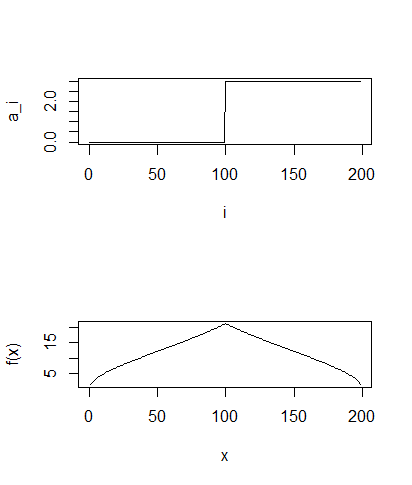
\includegraphics{Lemma2} %% graph doesn't work "no Lemma2 found"
%emph{a graph of $f$.}
%\end{figure}

The proof of the lemma is algebraic and won't be discussed. This lemma proves that if we have a function $f$ as defined above, then the maximum of $f$ must be attained at one of the \(a_i\) in the sum. This is useful to us as our family of statistics \(Z^k_{k_1, k_2}, W^k_{k_1, k_2}, \Theta^k_{k_1, k_2} \)have the same form as $f$; so by applying the lemma we know that the maximum of our statistic will occur at a change-point. The next lemma will prove this.
\end{lemma}
%
The following setup will be in use throughout Lemma 3.4 to Lemma 3.9. let \(k_1, k_2\) be such that \[\nu_{i_0} \leq k_1 < \nu_{i_0+1} < \cdots < \nu_{i_0+l} < k_2 \leq \nu_{i_0+l+1},\]

where \(0 \leq i_0 \leq m_n - l\), that is the number of change points between our upper and lower test bounds is atmost the total number of change-points minus the number of change-points outside the interval. Since the function \(\Theta\) as defined %from statistics definitions
is invariant under location shift we may assume without loss of generality that
\[M_{k_2} - M_{k_1} = 0.\]

Since a location shift doesn't affect the change-points, in the following lemmas when we refer to the mean of a random variable \(X_k\) within the context of segment \( \{ k_1 +1, \cdots, k_2 \} \), we deal not with the actual mean but the mean after a location shift so that the above equation holds.

\begin{lemma}
%
Let \( k_1, k_2 \) be such that equation (2.8) holds for some \(l > 0\). Then if \(|\Theta^k_{k_1,k_2}| = \Theta_{k_1,k_2}\), then \( k = \nu_{i_0+i}\) for some \(0 \leq i \leq l\).

Proof:\newline
Let \(a_i = (\nu_{i_0+i} - k_1)/(k_2 - k_1)\) and \(\theta_i = E[X_{\nu_{i_0+i}}]\). Then
\[ \Theta^k_{k_1,k_2} = f \Bigg(\frac{k - k_1}{k_2 - k_1}\Bigg ) \sqrt{k_2 - k_1}.\]

Now the result follows from Lemma 2.2.
\end{lemma}
%
%put something interesting in here


We need one or both of the following conditions on \(k_1, k_2\) in Lemmas 2.5 through 2.8.

\[s\].

The first condition is that the distance between change points within the interval \( [k_1, k_2]\) is atleast \(2cn^{1-\beta}\) and that the first and last change-point is atleast \(cn^{1-\beta} \) from \( k_1 \) and \( k_2 \) respectively.

The second condition is that the smallest of the maximum distances between the two closest change-points to \(k_1\) and \(k_2\) are atmost \(n^\alpha log \ n\).

\begin{lemma}
%
suppose \(k_1, k_2\) satisfy the above (2.10) and the conditions of the theorem hold.
Then
\[\max_{k_1<k<k_2}|\Theta^k_{k_1,k_2}| \geq \frac{\delta}{2}cn^{\frac{1}{2} - \beta}.\]

Proof: \newline
Let \(E[X_{\nu_i}] = \theta \ and \ E[X_{\nu_{i + 1}}] = \theta^{'}\). Since \(| \theta - \theta^{'}| > \delta\), by condition (\(ii\)) of the theorem, we get that
\[ |\theta| \vee |\theta^{'}| > \frac{\delta}{2}.\]

By the above inequality and the definition of $M_k$ (the partial sum of the means for \(X_i\)) up to $k$ we can see that

\[|M_{\nu_i} - M_{\nu_i - cn^{1-\beta}}| \vee |M_{\nu_i + cn^{1-\beta}} - M_{\nu_i}| > \frac{\delta}{2}cn^{1 - \beta}\]
%explaination required

From the (2.13) we get that the maximum of \(|M_k - M_{k_1}|\) is atleast \(\frac{\delta}{4}cn^{1-\beta}\). Finally since \[\frac{(k - k_1)(k_2 - k)}{k_2 -k_1} \leq \frac{(k_2-k_1)}{4} \leq \frac{n}{4}\] we get the lemma.

\end{lemma}

\begin{lemma}
Suppose \(k_1, k_2\) satisfy (2.10) and (2.11) for some \(\alpha < 1 -2\beta \). Let $\nu$ be a change-point that satisfies

\[ \Theta^\nu_{k_1, k_2} > \Theta_{k_1, k_2} - 6\sqrt{log n}.\]

Where \[\Theta^\nu_{k_1, k_2} = \frac{a}{\sqrt{\frac{(\nu - k_1)(k_2 - \nu)}{(k_2 - k_1)}}}\]. Then under the conditions of the theorem, for large n,

\[a > \frac{\delta cn^{1 - \beta}}{5}\]

Proof: \newline
Observe that
 \[\Theta^\nu_{k_1, k_2} = \frac{a}{\sqrt{\frac{(\nu - k_1)(k_2 - \nu)}{(k_2 - k_1)}}} \leq 2\sqrt{2}B\sqrt{(\nu -  k_1) \vee (k_2 - \nu)}.\]

Also \((\nu - k_1) \vee (k_2 - \nu)\) is either less than \(n^\alpha log n\) or larger than \(2cn^{1 - \beta} - n^\alpha log n\). Since by Lemma 2.5 the first possibility contradicts (2.14) (because \( \alpha < 1 - 2\beta\)), for large n, we get that

\[ (\nu -  k_1) \vee (k_2 - \nu) \geq 2cn^{1- \beta} - n^\alpha log n.\]

Without loss of generality we could assume that \(2(\nu - k_1) \leq (k_2 - k_1).\) Let \(\nu = \nu_{i_0 + i}\) for some \(1 \leq i \leq l\). Let $\theta$ and $\theta^{'}$ be the mean of $X_\nu$ and $X_{\nu + 1}$ respectively. Then by condition \((ii)\) of the theorem either $|\theta|$ and $|\theta^{'}|$ is greater than $\frac{\delta}{2}$.
\end{lemma}

\chapter{Consistency estimation}
%
The result analysed previously is a useful result however Fryzlewicz, Piotr et al showed that you can improve Binary segmentation by testing subsamples of the data chosen randomly%\cite{Wild}
. In this chapter we show the motivation for this result and use Monte Carlo methods to compute the ??consistency of Binary Segmentation??. %% obviously wrong needs rewording ask Haeron Cho
\section{Counter-example}
%
In some ways binary segmentation can" be considered a 'greedy' procedure in the sense that it is performed sequentially, with each stage depending on the previous ones"%% is a quote reword
As binary segmentation computes a global search on the dataset and each estimated change-point is accepted on the basis of one test, 
\chapter{Real world Application}
%%%%%%%%%% INFORMATION %%%%%%%%%%
\section{A Note About References}
%
The Third and Fourth Year Handbook, and the Third and Fourth Year Project Handbook, have some clear guidelines about plagiarism and referencing.
You should consult your project supervisor about the correct format for handling references.

This document uses the `in-text' or Harvard system of referencing, which is a good default format.
This requires both in-text citations and a list of references at the end of the document.
The project templates have an example of a list of references.

Within the text you must cite the authors surname(s) and the date of publication.
When referring to a specific idea, or a direct quote, you must also give the page number.
If there are two authors, use `and' and if there are more, use `et al.'\ and give all the authors names at the end.

There are two styles of citation, implicit and explicit.
Both are equally acceptable and it is also acceptable to mix and match.

\subsection{Examples of implicit in-text citations}
%
The sum of convex functions is itself convex (Blacke, 1985) and therefore any minimiser of this objective function will be a global minimiser (Greene and Whit, 1995, p.123). It is possible to exploit this fact (Browne et al., 2005) to enhance the optimisation algorithm.

\subsection{Examples of explicit in-text citations}
%
Blacke (1985) first proved that a sum of convex functions is convex. Any minimiser of this objective function will be a global minimiser, a fact shown by Greene and Whit (1995, p.123) and exploited by Browne et al.\ (2005) to enhance the optimisation algorithm.

%%%%%%%%%% APPENDIX %%%%%%%%%%
\appendix
\chapter{An Appendix may not be necessary}
%
Text introducing the/this appendix.

\section{Appendix section}
%
Text of this section.
$\mathbb{R}$
Subsections and further divisions can also be used in appendices.

%%%%%%%%%% BIBLIOGRAPHY %%%%%%%%%%
\bibliographystyle{plain}
\bibliography{mybib} { }

%


\end{document}
